\documentclass[UTF8]{ctexart}
\usepackage[paper=a4paper,dvips,top=2.5cm,left=2.8cm,right=2.8cm,foot=1cm,bottom=3.2cm]{geometry}
\usepackage{fancyhdr}
\usepackage{indentfirst}
\usepackage{enumerate}
\usepackage{amsfonts}
\usepackage{clrscode}
\usepackage{listings}
\usepackage{amsmath}
\usepackage{amstext}
\usepackage{algorithm}  
\usepackage{algorithmic}  
\renewcommand{\algorithmicrequire}{ \textbf{Input:}} %Use Input in the format of Algorithm  
\renewcommand{\algorithmicensure}{ \textbf{Output:}} %UseOutput in the format of Algorithm  
\DeclareMathOperator*{\argmin}{arg\,min}
\DeclareMathOperator*{\argmax}{arg\,max}
\renewcommand{\algorithmicprint}{\textbf{break}}
\lstset{language=Matlab}%代码语言使用的是matlab
\lstset{breaklines}%自动将长的代码行换行排版
\lstset{extendedchars=false}%解决代码跨页时,章节标题,页眉等汉字不显示的问题
\usepackage{graphicx}
\usepackage[colorlinks,linkcolor=blue,urlcolor = blue]{hyperref}
\DeclareGraphicsExtensions{.eps,.ps,.jpg,.bmp}
\pagestyle{plain}
\begin{document}
\par 尊敬的吴老师,您好
\newline 
\par
我完成了基于no-overlapping community的diffusion minimization problem的仿真,仿真结果与原文基本一致。此处的原文是指Information Diffusion in Mobile Social Networks:
The Speed Perspective(2014),与作者在2016年发表的Towards Information Diffusion in Mobile Social Networks的内容基本一致,不过2016的那篇是基于overlapping community的。下面先介绍论文内容,最后附上一些我的个人理解。
\subsection*{1. 问题描述}
最快传播问题:在网络中选择一个大小为k的节点集合,使得从该集合开始传播的信息能够以最短的时间扩散到整个网络。
\subsubsection*{1.1 网络模型}
\par 记$G=(V,E)$为有权无向图,其中$V$为节点集合,$E$为边集合。对于两个相邻节点$u,v \in V$,$w_{uv}$表示两点连边的权重,同时$w_{uv}=w_{vu}$。边的权重反映了节点之间的互动频率。对于节点$u \in V$,$d_u$表示节点$u$的度,$N_u$表示节点$u$的相邻节点集合,并且$d_u = \sum_{v \in N_{u}} w_{uv}$。
\subsubsection*{1.2 传播概率模型}
\par 在信息传播模型中,节点的状态可分为激活的和未激活的。激活的节点可以向其未激活的邻居传播信息。具体的,当一个已激活的节点$u$向未激活节点$v$传递信息时,节点$v$被激活的概率为$\lambda_{uv}=\frac {w_{uv}}{d_u}$。这是因为信息从$u$传播到它的邻居$v$的概率应该正比于$v$在$d_u$的比例。换句话说,$u$与$v$的互动越频繁,$v$越有可能被$u$激活。从社会关系的角度来说,人们更喜欢向最好的朋友分享信息,而不是其他人。
\subsubsection*{1.3 问题描述}
\par 信息传播的过程可以这样描述:首先选择一个初始的已激活节点集合,随着已激活节点与未激活节点的互动交流,未激活节点以一定概率被激活,当所有节点都被激活时,传播过程结束。
\par 记$S$为初始化节点集合,$S$的传播时间定义为传播过程开始至结束的时间间隔,记为$\tau (S,V)$。
\par 在给定图$G=(V,E)$和一个整数$k$后,我们的目的是确定一个节点集合$S$,$\left | S  \right |\leq k$且$S \subseteq V$,使得$\tau (S,V)$为最小。这个问题通常被称为最小传播问题(diffusion minimization)。
\par 节点$u$到节点$v$的期望传播时间记为
\begin{equation}
\label {equ:1}
t_{uv}=\frac {1}{\lambda_{uv}} \cdot \frac {1} {w_{uv}} = \frac {d_u}{w_{uv}} \cdot \frac {1}{w_{uv}}=\frac {d_u}{w^{2}_{uv}}
\end{equation}
其中$\frac {1}{w_{uv}}$表示传播的平均时间间隔。对于任何节点对,例如节点$u$和$v$,$u$至$v$的最短期望传播时间记为$\left | (u,v)  \right |$,为了简化描述,不妨称$\left | (u,v)  \right |$为节点$u$至$v$的期望传播时间。
\par 最小传播问题可以这样表述:寻找一个集合$S \subseteq V$($\left | S  \right |\leq k$),使得期望传播时间$\tau (S,V)$:
\begin{equation}\tau'(S,V) = \min \max_{v \in V} \left | (S,v)  \right | \label{equ:2} \end{equation}
其中
\begin{equation}\left | (S,v)  \right | = \min_{u \in S} \left | (u,v)  \right | \label{equ:3}\end{equation}
$\left | (S,v)  \right |$是集合$S$至节点$v$的期望传播时间。
\subsubsection*{1.4 一个朴素算法}
\par 节点的紧密度(closeness)是该节点至所有其他节点的最短路径长度之和的倒数,例如节点$u$的紧密度为$1 \setminus \sum_{v \in V} \left | (u,v) \right |$。
\par 紧密度可以看作是节点传播信息速度的度量,紧密度越大,传播速度越快。我们可以不断地从$V\setminus S$中选取最大紧密度的节点加入集合$S$,直至$\left | S  \right |=k$。具体的,每次选取过程中节点$u$的紧密度这样计算
\begin{equation}\frac {1}{\sum_{v\in V \setminus S} \left | (u,v)  \right |}, \, u \notin S \label{equ:4}\end{equation}
\subsection*{2 社区化算法}
\par 相比于社区外部节点,社区内部的节点之间连接关系更多。社区结构清晰地表示了节点如何组织以及节点之间如何互动。在信息传播方面,社区有如下属性:
\begin{enumerate}[\indent 1)]
\item 在社区内部,节点互动频繁,信息可以快速传播。
\item 信息在社区之间的传播速度远比社区内部慢。
\end{enumerate}
\par 最基本的社区化算法是在每个社区内部至少选取一个传播节点。记$\mathfrak{C} = \left \{ C_1,C_2,C_3,\cdots,C_l \right \}$为社区列表,其中$\left | \mathfrak{C}  \right |=l$,$C_i \in \mathfrak{C}$表示一个社区。假设需要在$\mathfrak{C}$中确定$k$个节点,这里有两种情况:$k<l$和$k\geq l$。对于$k<l$,我们不能保证每个社区中都至少有一个初始传播节点,因此一些社区需要合并。对于$k \geq l$,我们要考虑如何在一个社区中选择多个初始传播节点。所以,接下来我们首先介绍如何合并社区,以确保$k\geq l$,然后介绍如何在一个社区中选择多个初始传播节点。

\subsubsection*{2.1 社区合并}


\par 社区中心节点是在社区内部,对所有其他节点具有最小期望传播时间的节点。社区中心节点的期望传播时间称为社区传播半径。

\par 记$N_C$和$R(C)$为社区中心节点和社区传播半径,并且
\begin{equation}R(C) = \min_{u \in C}(\max_{v \in C}\left | (u,v) \right |)\label{equ:5}\end{equation}

\par 通过社区合并,社区数量会从$l$减少至$k$。之后,整个网络的期望传播时间由具有最大传播半径的社区决定。所以在社区合并的过程中,我们应该最小化$\max \left \{ R(C):C \in \mathfrak(C) \right \}$。显然,$R(C_i \cup C_j) > \max\left \{R(C_i),R(C_j)\right \}$。因此被合并的社区的传播半径会扩大。我们每次需要合并两个社区,有$\begin{pmatrix}
\left |\mathfrak{C}  \right |\\ 
2
\end{pmatrix}$种选择,显然直接枚举行不通。

\par 一种可行的社区合并方法是合并相邻的社区,使得合并后的社区的传播半径尽可能小。如果$C_j$满足公式\eqref{equ:6},则称$C_j$为$C_i$的相邻社区。$C_i$的相邻社区集合记为$\mathfrak{C}_{C_i}$
\begin{equation}\mathfrak{C}_{C_i} = \left \{ C_j \in \mathfrak{C} \setminus \left \{ C_i \right \}:\frac {\sum_{u \in C_i,v\in C_j} w_{uv} } {\left | C_{j} \right | } \geq 
\frac {\sum_{u \in C_i,v\in V \setminus C_i} w_{uv} } {\left | V \setminus C_{j} \right | } \right \}\label{equ:6}\end{equation}

\par 社区合并过程如下:首先,我们在$\mathfrak{C}$选择具有最小传播半径的社区$C_i$;从$C_i$的相邻社区集$\mathfrak{C}_{C_i}$中选择$C_j$,使得$R(C_i \cup C_j)$最小,如果$R(C_i \cup C_j) \leq \max\left \{ R(C):C\in \mathfrak{C} \right \}$,那么合并$C_i$和$C_j$,否则,遍历所有其他的社区。如果找不到满足$R(C_i \cup C_j) \leq \max\left \{ R(C):C\in \mathfrak{C} \right \}$的社区,选择具有最小$R(C_i \cup C_j)$的社区$C_i$和$C_j$来进行合并。具体算法过程见Algorithm \ref{alg:Merging}。
\begin{algorithm}[htb]   
\caption{ Community Merging}   
\label{alg:Merging}   
\begin{algorithmic}[1] %这个1 表示每一行都显示数字  
\REQUIRE ~~ %算法的输入参数:Input  
$\mathfrak{C}$ 
\ENSURE ~~ %算法的输出:Output  
$\mathfrak{C}$
\label{ code:fram:extract }%对此行的标记,方便在文中引用算法的某个步骤  
\WHILE{$\left | \mathfrak{C} \right | > k $}
\STATE $\mathfrak{C}' = \mathfrak{C}$
\STATE $C_i=C_j=\O $
\WHILE{$\left | \mathfrak{C}' \right | $}
\STATE $C_{i}' = \argmin_{C \in \mathfrak{C}'}R( C)$
\STATE $C_{j}' = \argmin_{C \in \mathfrak{C}_{C_i}'}R(C_i \cup C)$
\IF{$R(C_{i}' \cup C_{j}') < \max \left \{ R(C): C\in \mathfrak{C} \right \}$}
\STATE $C_{i} = C_{i}'$ and $C_j = C_{j}'$ 
\PRINT
\ELSE
\IF{$R(C_{i} \cup C_{j}) \leq R(C_{i}' \cup C_{j}') $}
\STATE $C_{i} = C_{i}'$ and $C_j = C_{j}'$ 
\ENDIF
\STATE $\mathfrak{C}' = \mathfrak{C}' \setminus \left \{ C_{i}' \right \}$
\ENDIF
\ENDWHILE
\STATE $\mathfrak{C} = \mathfrak{C} \setminus \left \{ C_i,C_j\right \} \cup \left \{ C_i \cup C_j\right \}$
\ENDWHILE 
\end{algorithmic}  
\end{algorithm}   

\subsubsection*{2.2 确定初始传播节点}

\par 经过社区合并后,$\left | \mathfrak{C} \right | \leq k$,因此我们需要在一个社区内确定多个传播节点。
\par 记$S_{C_i}$为$C_i$中的初始传播集合,记$\left | (S_{C_i},u) \right |$为$S_{C_i}$至节点$u \in C_i$的期望传播时间。为了在社区内确定多个初始传播节点,我们按照公式\eqref{equ:7}来迭代选择节点$u$加入集合$S_{C_i}$
\begin{equation}
\argmin_{u \in C_i \setminus S_{C_i}}  \sum_{v \in C_i \setminus S_{C_i}} \left |(S_{C_i} \cup \left \{ u \right \},v) \right |
\label{equ:7}\end{equation}
$S_{C_i}$选择完成后,社区$C_i$的期望传播时间记为$\tau'(S_{C_i},C_{i})$

\subsubsection*{2.3 算法设计}

\par 合理的选择初始传播节点可以有效地减少传播时间。一种最直接的方法是先为每个社区选择中心节点,然后迭代地在满足$R(C):C \in \mathfrak(C)$的社区中选择初始传播节点,直至$\left | S \right | = k$。然而,这种方法并不总是有效的。举例来说,$\mathfrak{C}$中有原始社区$C_i$,已合并社区$C_j$和$C_k$,且$R(C_i) > \max \left \{ R(C_j),R(C_k) \right \}$。那么显然在$C_i$中选择多个初始节点,在$C_j$和$C_k$中各选择一个初始节点更优。
\par 社区化算法工作流程如下。首先我们先合并社区,直至$\forall C_i,C_j:R(C_i \cup C_j)> \max \left \{ R(C):C \in \mathfrak(C) \right \}$;然后,我们为每个选择中心节点作为初始传播节点,这样我们仍有$k-\mathfrak(C)$个初始传播节点待定;接下来,我们为具有最大传播半径的社区$C_i$选择额外的初始传播节点。如果$C_i$是已合并社区,那么将$C_i$分裂为社区$C_j$和$C_k$,用$C_j$和$C_k$的中心节点替代$C_i$的中心节点。如果$C_i$是原始社区,那么我们先根据公式\eqref{equ:7}选取一个初始传播节点来代替$N_{C_i}$,然后在确定更多的初始传播节点,并加入集合$S$。算法细节见Algorithm \ref{alg:Community}。
\begin{algorithm}[htb]   
\caption{ Community based Algorithm}   
\label{alg:Community}   
\begin{algorithmic}[1] %这个1 表示每一行都显示数字  
\REQUIRE ~~ %算法的输入参数:Input  
$\mathfrak{C}$ 
\ENSURE ~~ %算法的输出:Output  
$S$
\label{ code:fram:extract }%对此行的标记,方便在文中引用算法的某个步骤 
\STATE  $\mathfrak{C}' = \mathfrak{C}$
\WHILE{$\exists C_i,C_j:R(C_i \cup C_j) < \max_{C \in \mathfrak{C}'}R(C)$}
\STATE $\mathfrak{C}' = \mathfrak{C}'\setminus \left \{ C_i,C_j\right \} \cup \left \{ C_i \cup C_j\right \}$
\ENDWHILE
\STATE $S = \left \{N_C:C \in \mathfrak{C}' \right \}$
\WHILE{$\left | S \right | < k$}
\STATE $C = \argmax_{C\in \mathfrak{C}'}R(C)$
\IF{$C \in \mathfrak{C}$}
\IF{$\left | S_{C} \right | = 1$}
\STATE $S = S \setminus \left \{ N_C \right \}$
\STATE $S = S \cup \left \{ \argmin_{u \in C \setminus S_C} \sum_{v \in C \setminus S_C} \left | (S_C \cup \left \{u \right \},v ) \right | \right \}$
\ENDIF
\STATE $S = S \cup \left \{ \argmin_{u \in C \setminus S_C} \sum_{v \in C \setminus S_C} \left | (S_C \cup \left \{u \right \},v ) \right | \right \}$
\ELSE
\STATE $S = S \cup \left \{ N_C \right \} \cup \left \{ N_{C_i},N_{C_j} \right \}$
\STATE $\mathfrak{C}' = \mathfrak{C}' \setminus \left \{ C \right \} \cup \left \{ C_i \cup C_j\right \}$
\ENDIF
\ENDWHILE
\end{algorithmic}  
\end{algorithm}  
\subsection*{3 仿真实验}
\par 我们将在人工合成数据集上对比社区化算法(Community)和朴素算法(Naive),数据集来自于Benchmark程序,其参数列表如表\ref{Parameter}所示。其中$n$为节点数量,$\alpha$为节点邻居数量,$\alpha_{max}$为节点最大邻居数量,$\mu_w$为边权重混合度,$\mu_t$为图拓扑混合度,$\varepsilon_1$为节点度的最小幂,$\varepsilon_2$为社区大小分布的最小幂,$\beta$为权重分布最小幂。
\begin{table}[H]
\centering
\begin{tabular}{|c|c|c|c|}
\hline
\textbf{Parameter} & \textbf{Value} & \textbf{Parameter} & \textbf{Value}  \\
\hline
\hline
$n$ & 500,1000,2000 & $\varepsilon_1$  & 2  \\
$\mu_w$ & 0.1,0.3 &  $\varepsilon_2$ & 1  \\
$\mu_t$ & 0.1,0.3 &  $\alpha$ & 15 \\
$\beta$ & 2       & $\alpha_{max}$   &  20 \\
\hline
\end{tabular}
\caption{benchmark 参数设置}
\label{Parameter}
\end{table} 
\par 图\ref{fig-res}展示了社区化算法和朴素算法在不同网络参数下的期望传播时间。在实际应用中,$k$通常是一个较小值,在这里我们选取的$k$值不会超过网络节点数的$5\%$。
\begin{figure}[H]
    \centering
    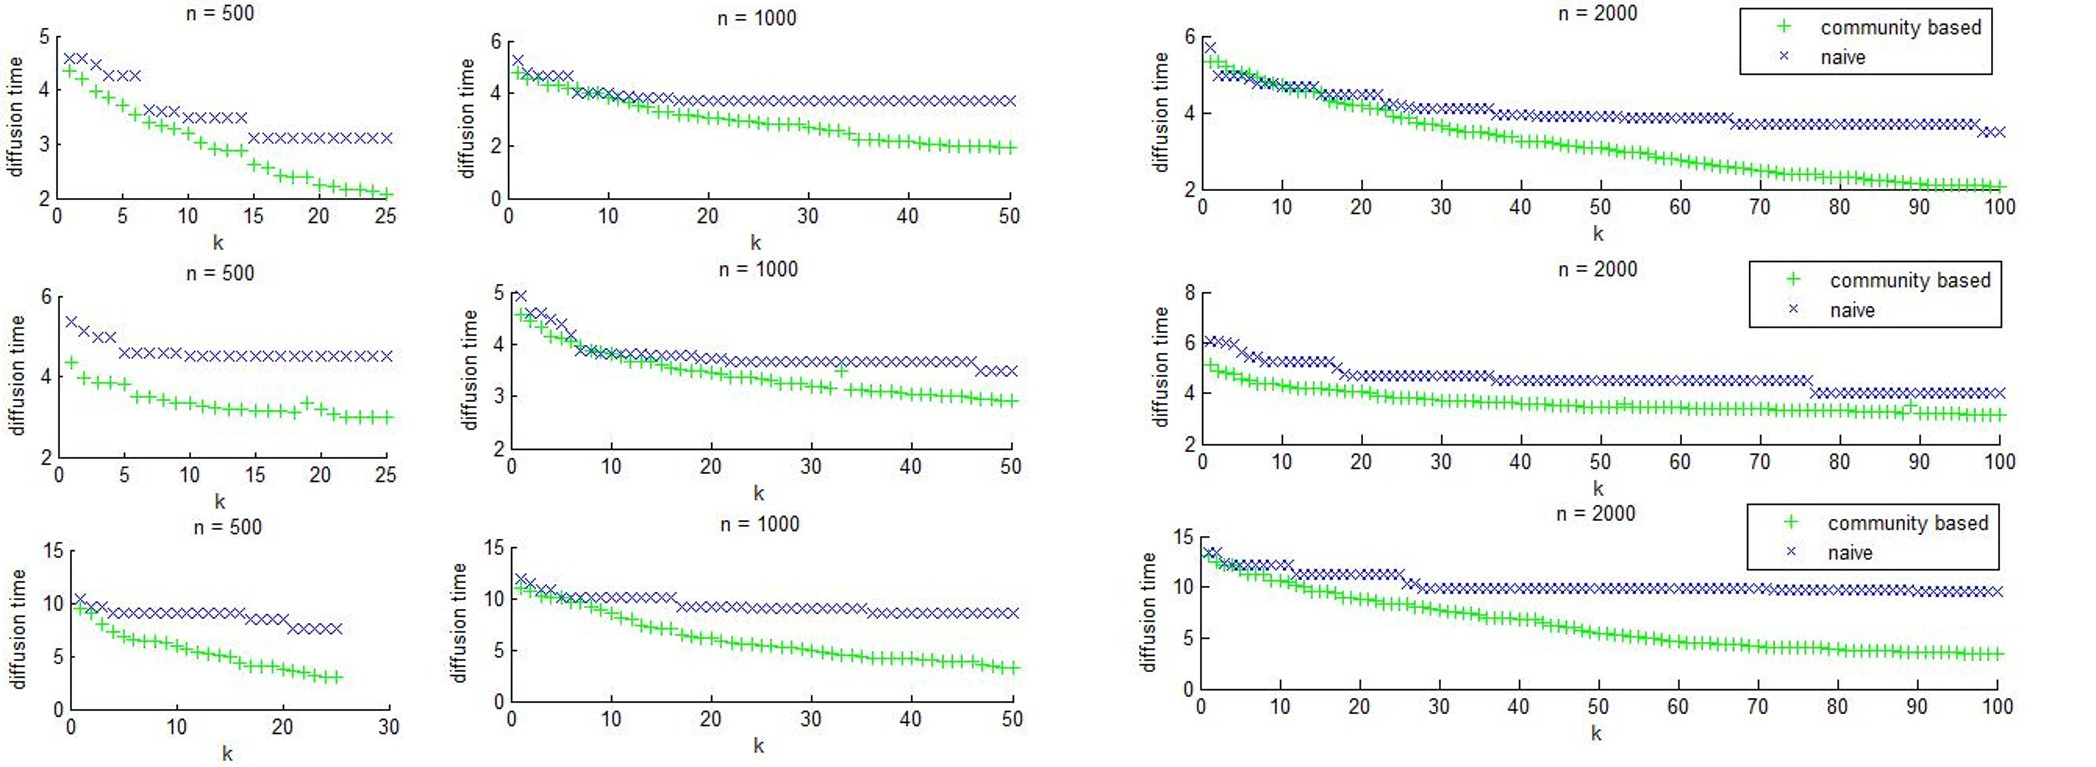
\includegraphics[width=16cm]{fig-res.jpg}
    \caption{Community vs Naive}
    \label{fig-res}
\end{figure}

\subsection*{4 补充说明}
\par 作者在公式\eqref{equ:1}中说明了如何计算两个相邻节点的期望传播时间,但关于如何计算任意两个节点的期望传播时间未做说明。我这里用了Dijkstra算法得到所有节点对的最短路径权值矩阵$M$,其中$M_{uv}$表示节点$u$到$v$的期望传播时间$\left |(u,v) \right |$。这样对于公式\eqref{equ:3}而言,其实就是对矩阵$M$的某些行的所有元素求最大;对于公式\eqref{equ:4}而言,则是对矩阵$M$的某一行求和取倒数;而公式\eqref{equ:5}则是对矩阵$M$的某些行先求行最大,再对结果求最小;公式\eqref{equ:7}是对矩阵$M$的某些行的所有元素求和。
\par 我是用C++写的程序,对于规模为500,1000,2000的网络,运行时间大致为1s,1-5mins,20-60mins,并且时间都消耗在了Dijkstra算法上面。程序代码见\url{https://github.com/Chaomin702/Community}。
\newline
\par \textbf{接下来我想去做}
\begin{enumerate}[\indent 1)]
\item 基于overlapping community的最小传播问题仿真。
\item distributed set-cover algorithm仿真
\end{enumerate}

\par \rightline{学生王超民,2016年10月14日}
\end{document}
